\documentclass[conference]{IEEEtran}
\IEEEoverridecommandlockouts
% The preceding line is only needed to identify funding in the first footnote. If that is unneeded, please comment it out.
\usepackage{cite}
\usepackage{amsmath,amssymb,amsfonts}
\usepackage{algorithmic}
\usepackage{graphicx}
\usepackage{textcomp}
\usepackage{xcolor}
\def\BibTeX{{\rm B\kern-.05em{\sc i\kern-.025em b}\kern-.08em
    T\kern-.1667em\lower.7ex\hbox{E}\kern-.125emX}}
\begin{document}

\title{Effect of Injection and Valve Timing on Combustion Characteristics and Performance of Port-Fuelled Hydrogen Internal Combustion Engines
}

\author{\IEEEauthorblockN{Isuru Wickramaarachchi}
\IEEEauthorblockA{\textit{Department of Mechanical Engineering} \\
\textit{University of Moratuwa}\\
Katubedda, Sri Lanka \\
waisurumangala@gmail.com}
\and
\IEEEauthorblockN{Isuru Wickramaarachchi}
\IEEEauthorblockA{\textit{Department of Mechanical Engineering} \\
\textit{University of Moratuwa}\\
Katubedda, Sri Lanka \\
waisurumangala@gmail.com}
\and
\IEEEauthorblockN{Isuru Wickramaarachchi}
\IEEEauthorblockA{\textit{Department of Mechanical Engineering} \\
\textit{University of Moratuwa}\\
Katubedda, Sri Lanka \\
waisurumangala@gmail.com}
\and
\IEEEauthorblockN{Isuru Wickramaarachchi}
\IEEEauthorblockA{\textit{Department of Mechanical Engineering} \\
\textit{University of Moratuwa}\\
Katubedda, Sri Lanka \\
waisurumangala@gmail.com}
\and
\IEEEauthorblockN{Isuru Wickramaarachchi}
\IEEEauthorblockA{\textit{Department of Mechanical Engineering} \\
\textit{University of Moratuwa}\\
Katubedda, Sri Lanka \\
waisurumangala@gmail.com}
}

\maketitle

\begin{abstract}
The urgency to mitigate global warming has propelled hydrogen to the forefront as a viable alternative fuel. Hydrogen internal combustion engines, abnormal combustion poses a significant challenge. Manipulating design parameters such as valve timing, injection timing, and others can potentially mitigate this issue. The relationship between these adjustments and their impact on combustion characteristics and engine performance is not fully understood. Particularly, valve and injection timing are critical in influencing mixture formation—a determinant of combustion behavior and engine performance. Previous research has primarily focused on the isolated effects of these parameters, leaving a gap in understanding their synergistic influence. Our focus is to bridge this knowledge gap by comprehensively analyzing the combined effect of valve and injection timing on the combustion characteristics and performance of port-fueled hydrogen internal combustion engines. The combined effect of valve and injection timing on combustion characteristics and engine performance is investigated using numerical simulations.
\end{abstract}

\begin{IEEEkeywords}
valve timing, injection timing, performance, combustion characteristics, hydrogen
\end{IEEEkeywords}

\section{Introduction}
Global warming presents the most severe environmental challenge today, primarily driven by the increased carbon dioxide (CO2) emissions from the consumption of fossil fuels. The transportation sector, which heavily relies on Internal Combustion Engines (ICEs), remains a major contributor to these emissions. Consequently, the urgency to make these engines more sustainable and environmentally friendly is undeniable. Efforts to address this issue led to exploring the adoption of alternative fuels. In this regard, hydrogen has emerged as a compelling option, taking advantage of its favourable combustion characteristics together with zero carbon emissions. 
The literature identifies two distinct types of hydrogen engines: Port Fuel Injection (PFI) and Direct Injection (DI) engines. PFI involves injecting fuel into the intake manifold, where it mixes with air before reaching the combustion chamber. In contrast, DI engines inject hydrogen directly into the chamber during the compression stroke, initiating the ignition of the compressed air-fuel mixture. Particularly, in DI engines, the processes of fuel-air mixing, and combustion occur simultaneously, leading to less time available for mixture formation. To achieve sufficient mixing, higher injection pressures and precisely manufactured injectors are required, which leads to increased costs. Conversely, PFI separates the mixing and combustion processes, affording more time for the creation of a uniform fuel-air mixture, eliminating the necessity for precisely manufactured injectors and the application of high injection pressures. Therefore, PFI hydrogen engines represent a more viable solution for the rapid adaptation of alternative fuels due to their cost-effectivity and simple construction.
Abnormal combustion including knocking and backfire are major problems found in hydrogen engines. It has been demonstrated that those can be controlled by changing design parameters including valve timing, injection timing, injection pressure, intake pressure, spark timing and other parameters. Among the other parameters, valve and injection timing heavily affect the trapped hydrogen mass and mixture formation, which defines the combustion characteristics of internal combustion engines. The combustion process can lead to incomplete combustion or knocking combustion depending on the equivalence ratio.
Although valve and injection timing are individually studied, their influence on each other is highly undeniable. Both these parameters collectively define the mixture and thereby combustion characteristics and performance. Our project focuses on analyzing the combined effect of valve and injection timing on combustion characteristics and performance of port-fueled hydrogen internal combustion engines.


\section{Litreture Review}

\subsection{Injection Timing}

Wang [1] changed injection start times and monitored the hydrogen mass within the cylinder with crank angle. The amount of trapped mass and mass backflow was different under each scenario. Early injection caused less amount of backflow and higher fraction of mass can flow into the cylinder. Backflow of hydrogen can be seen in every case after the compression stroke starts (after 540 CAD). It can be explained using the push generated by the upward movement of the piston. If the hydrogen injection is delayed, more hydrogen mass would be affected by this negative force, consequently reducing trapped hydrogen mass. Yun [2] has also measured the trapped hydrogen mass but considering the wider range of injection timing. In addition to the decreasing trend of trapped mass with delayed hydrogen injection the effect of excessively early injection also identified. In combination, trapped hydrogen mass first increased and then decreased with change of injection timing. An optimum injection timing to trap maximum amount of hydrogen mass could be observed. Yun [2] also showed that the variation of indicated power and thermal efficiency were highly corelated with trapped hydrogen mass. In summary, to achieve higher engine performance, trapped hydrogen mass should be maximized. It could be achieved by careful variation of injection timing.
Literature gives evidence of forming locally concentrated hydrogen mass near inlet valve seats due to improper injection timing. Duan [3] showed that local concentration first increases and then decreases with injection delaying. When the injection is too early, hydrogen enters the inlet port and spreads towards the inlet valve before the valve opens. When the injection is too late, hydrogen injection continuous after the intake valve closes, causing high concentration mixture. Liu [4] also showed this increasing trend of local concentration with excessively delayed injection timing. 

Backfire as an abnormal combustion phenomenon, usually characterized by increased intake manifold pressure. Liu [3] showed in the same study of local concentration, excessively early or delayed injection also increases the maximum pressure in the intake port. In the intermediate injection times, the pressure rise is minimal. Comparison of local concentration of hydrogen mass and intake manifold pressure implies that local concentration of hydrogen near valve seats can strongly influence the backfiring risk. Therefore, local hydrogen concentration can be used to comment on the backfire possibility in port fueled hydrogen engines.

In brief, literature suggests that trapped hydrogen mass should be maximized to increase performance of the engine while keeping the local concentrations near inlet valve seats at a minimum level to prevent backfire risks.

    
\subsection{Valve Timing}

From the study [5] we can observe that both trapped mass and backflow mass with change of with valve timing. When the engine speed was lower than 2000 rpm, delaying Inlet Valve Close (IVC) causes a reduction in cylinder mass. The behavior is opposite with engine speeds higher than 2000 rpm. With early IVC, backflow mass was insignificant compared to cylinder mass. However, it is significant when the IVC is retarded. Higher backflow increases the local concentration near inlet valves, increasing the possibility of backfire. Since valve timing affects both trapped mass and local hydrogen concentrations, it is an important factor for both combustion characteristics and engine performance.
Park [6] showed the effect of Inlet Valve Open (IVO) timing on engine performance and efficiency for engine speed of 2000 rpm. Torque had a decreasing trend with retarding IVO, while the efficiency first increased before decreasing. This increase of thermal efficiency during the first half of IVO delay was due to the decrease in trapped mass. Huynh [7] studied a wider range valve overlap range from 00 - 500 to evaluate engine performance and showed that brake torque reduces in both low and excessive Valve Overlap Times (VOTs). Reduction of engine performance was much more significant with low VOTs than with high VOTs. VOT of 300 was shown to be the optimum VOT for the engine operating conditions in the study. The study also showed that, probability of backfire decreases with decrease of valve overlap. Backfire limiting equivalence ratio, increased up to 1.2 with zero valve overlap. This idea of backfire controlling with reducing VOT is also mentioned by Lee [8]. The study conducted experiments to show that IVO timing can be used to control backfire with an ultra-lean mixture. Results revealed that with a delay of 100CA, backfire-free operation can be ensured. 


\subsection{Combined Effect}

From the evidence above, trapped hydrogen mass and local concentration are highly dependent on both valve and injection timing. As [7] stated, combustion characteristics are changed due to mixing and turbulent intensities. Flow characteristics including turbulent intensities changes the amount of mixing thus the mixture uniformity. Proper mixing reduces the local pockets of high concentrated hydrogen which would otherwise cause abnormal combustion events.
This flow characteristics and mixture uniformity are highly influenced by the combined effect of both valve and injection timing. Further, since the trapped mass is affected by both valve and injection timing their combined effect is important to trap the correct amount of hydrogen mass within the cylinder, which would give proper combustion characteristics, performance, and efficiency. The combined effect on combustion characteristics and performance is not well demonstrated yet.

The importance of investigating the combined effect of valve and injection timing is mentioned by several researchers. [x, x, x, x].

\section{Engine Specifications}
Geometric and technical details are show in table 1.
\begin{table}[!ht]
    \centering
    \caption{Engine Specifications}
    \label{your_label_here}
    \begin{tabular}{|c|c|}
    \hline
    Header 1 & Header 2 \\
    \hline
    Bore & 92.6 mm \\
    Stroke & 86 mm \\
    Compression Ratio & 10.5 \\
    Equivalence Ratio & 0.59 \\
    Injection Duration & 155 CAD \\
    Engine Speed & 2000 RPM \\
    \hline
    \end{tabular}
    \end{table}

\section{Methodology}
\begin{itemize}
    \item Development of a validated numerical model.
    \item Analyze combustion characteristics with varying injection timing for the case of VOT = 300 to find suitable ranges of hydrogen injection.
    \item Evaluate combustion characteristics and performance for the range of valve and injection timing.
    \item Identify the combined effect of valve and injection timing on combustion characteristics and performance
\end{itemize}


\section{Numerical Model}
\subsection{Model Description}
Combustion models contain three regions including intake, cylinder, and exhaust. Redlich-Kwong gas equation is used for gas simulations. The Connaire reaction mechanism is used to calculate reaction rates. CFL number-based time stepping is used. The PISO algorithm is used for pressure velocity coupling. URANS-RNG k-epsilon model is used for turbulence modelling. O’Rourke and Amsden model are used to model wall heat transfer. For combustion modeling SAGE detailed chemistry solver is used. A high temperature energy source is used to model the ignition process while fuel injection is modelled as a mass inflow boundary condition.
\subsection{Mesh Sensitivity Analysis}
With the available computational power and license requirements, the maximum element count that we can run our simulations is 0.5 million. Mesh sensitivity analysis is carried out up to that point. The analysis shows that the mesh configuration with 8 mm base mesh is suitable for the analysis. The error compared to 6 mm base mesh configuration is only X percent.
\begin{figure}[htbp]
    \centerline{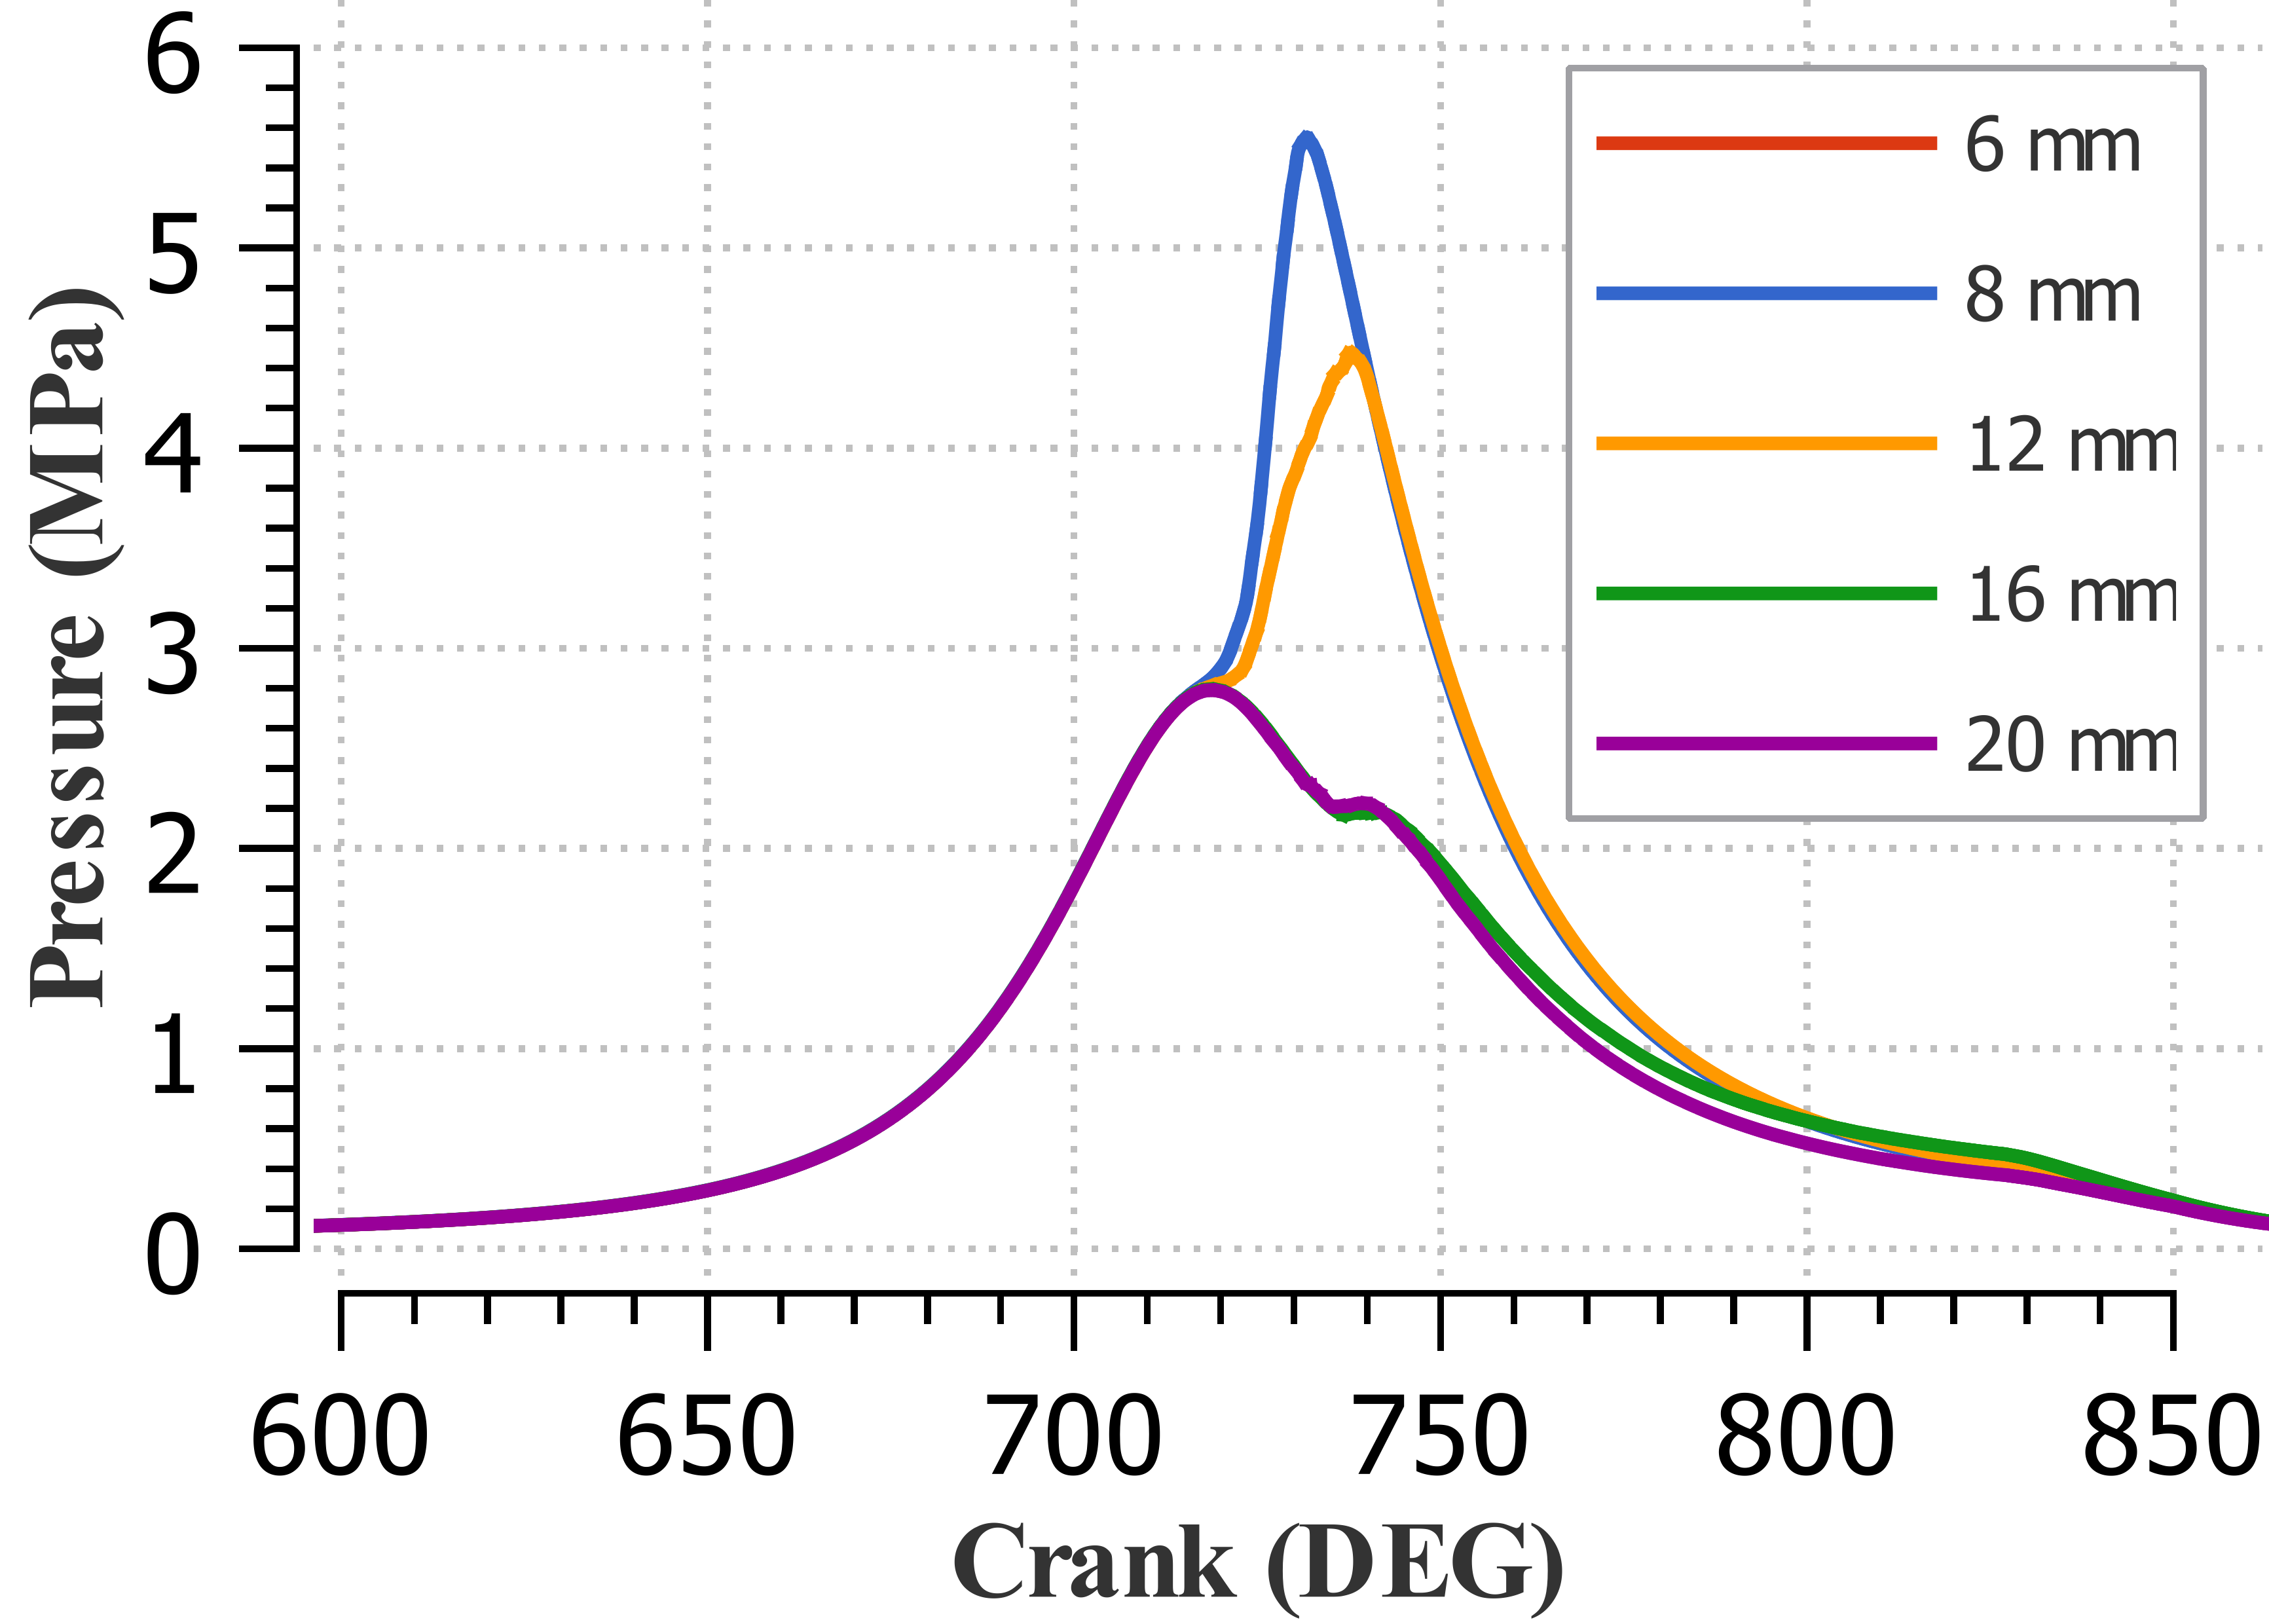
\includegraphics{Plots/mesh_sens.png}}
    \caption{Mesh Sensitivity}
    \label{plt_t}
    \end{figure}
\subsection{Model Validation}
As [4] also mentioned, simulation results are usually greater than experimental data due to limitations of computational mesh and from the fact that only one cylinder is modelled. Other than that, differences in the engine geometry also leads to deviation of results.
Although the maximum pressure differs by x percent, the numerical model follows the same trend as the experimental data. Therefore, this model can be used to find trends of the combustion process.

In the previous figure, we can see that the model is vlaidated.
    
\section{Analysis}
\subsection{Range Selection}
Valve overlap time range of 15-45 is selected for the analysis. reasons
VOT of 30 is first assumed to find the suitable range of injection timing with respect to intake valve open time, since VOT of 30 demonstrated the optimal engine performance in the study [7].
Range of start angles of 00 aIVO to 400 aIVO is tested for their combustion characteristics. 
It could be observed that, to properly combusts the mixture within the chamber while generating useful work injection start time of 200 aIVO to 300 aIVO is selected as possible range of injection.
Earlier injection leads knocking combustion while delayed injection leads to incomplete combustion.
Within the range injection start angles of 200 aIVO, 250 aIVO and 300 aIVO were selected as early, balanced, and delayed injection for all VOT values.

\begin{figure}[htbp]
    \centerline{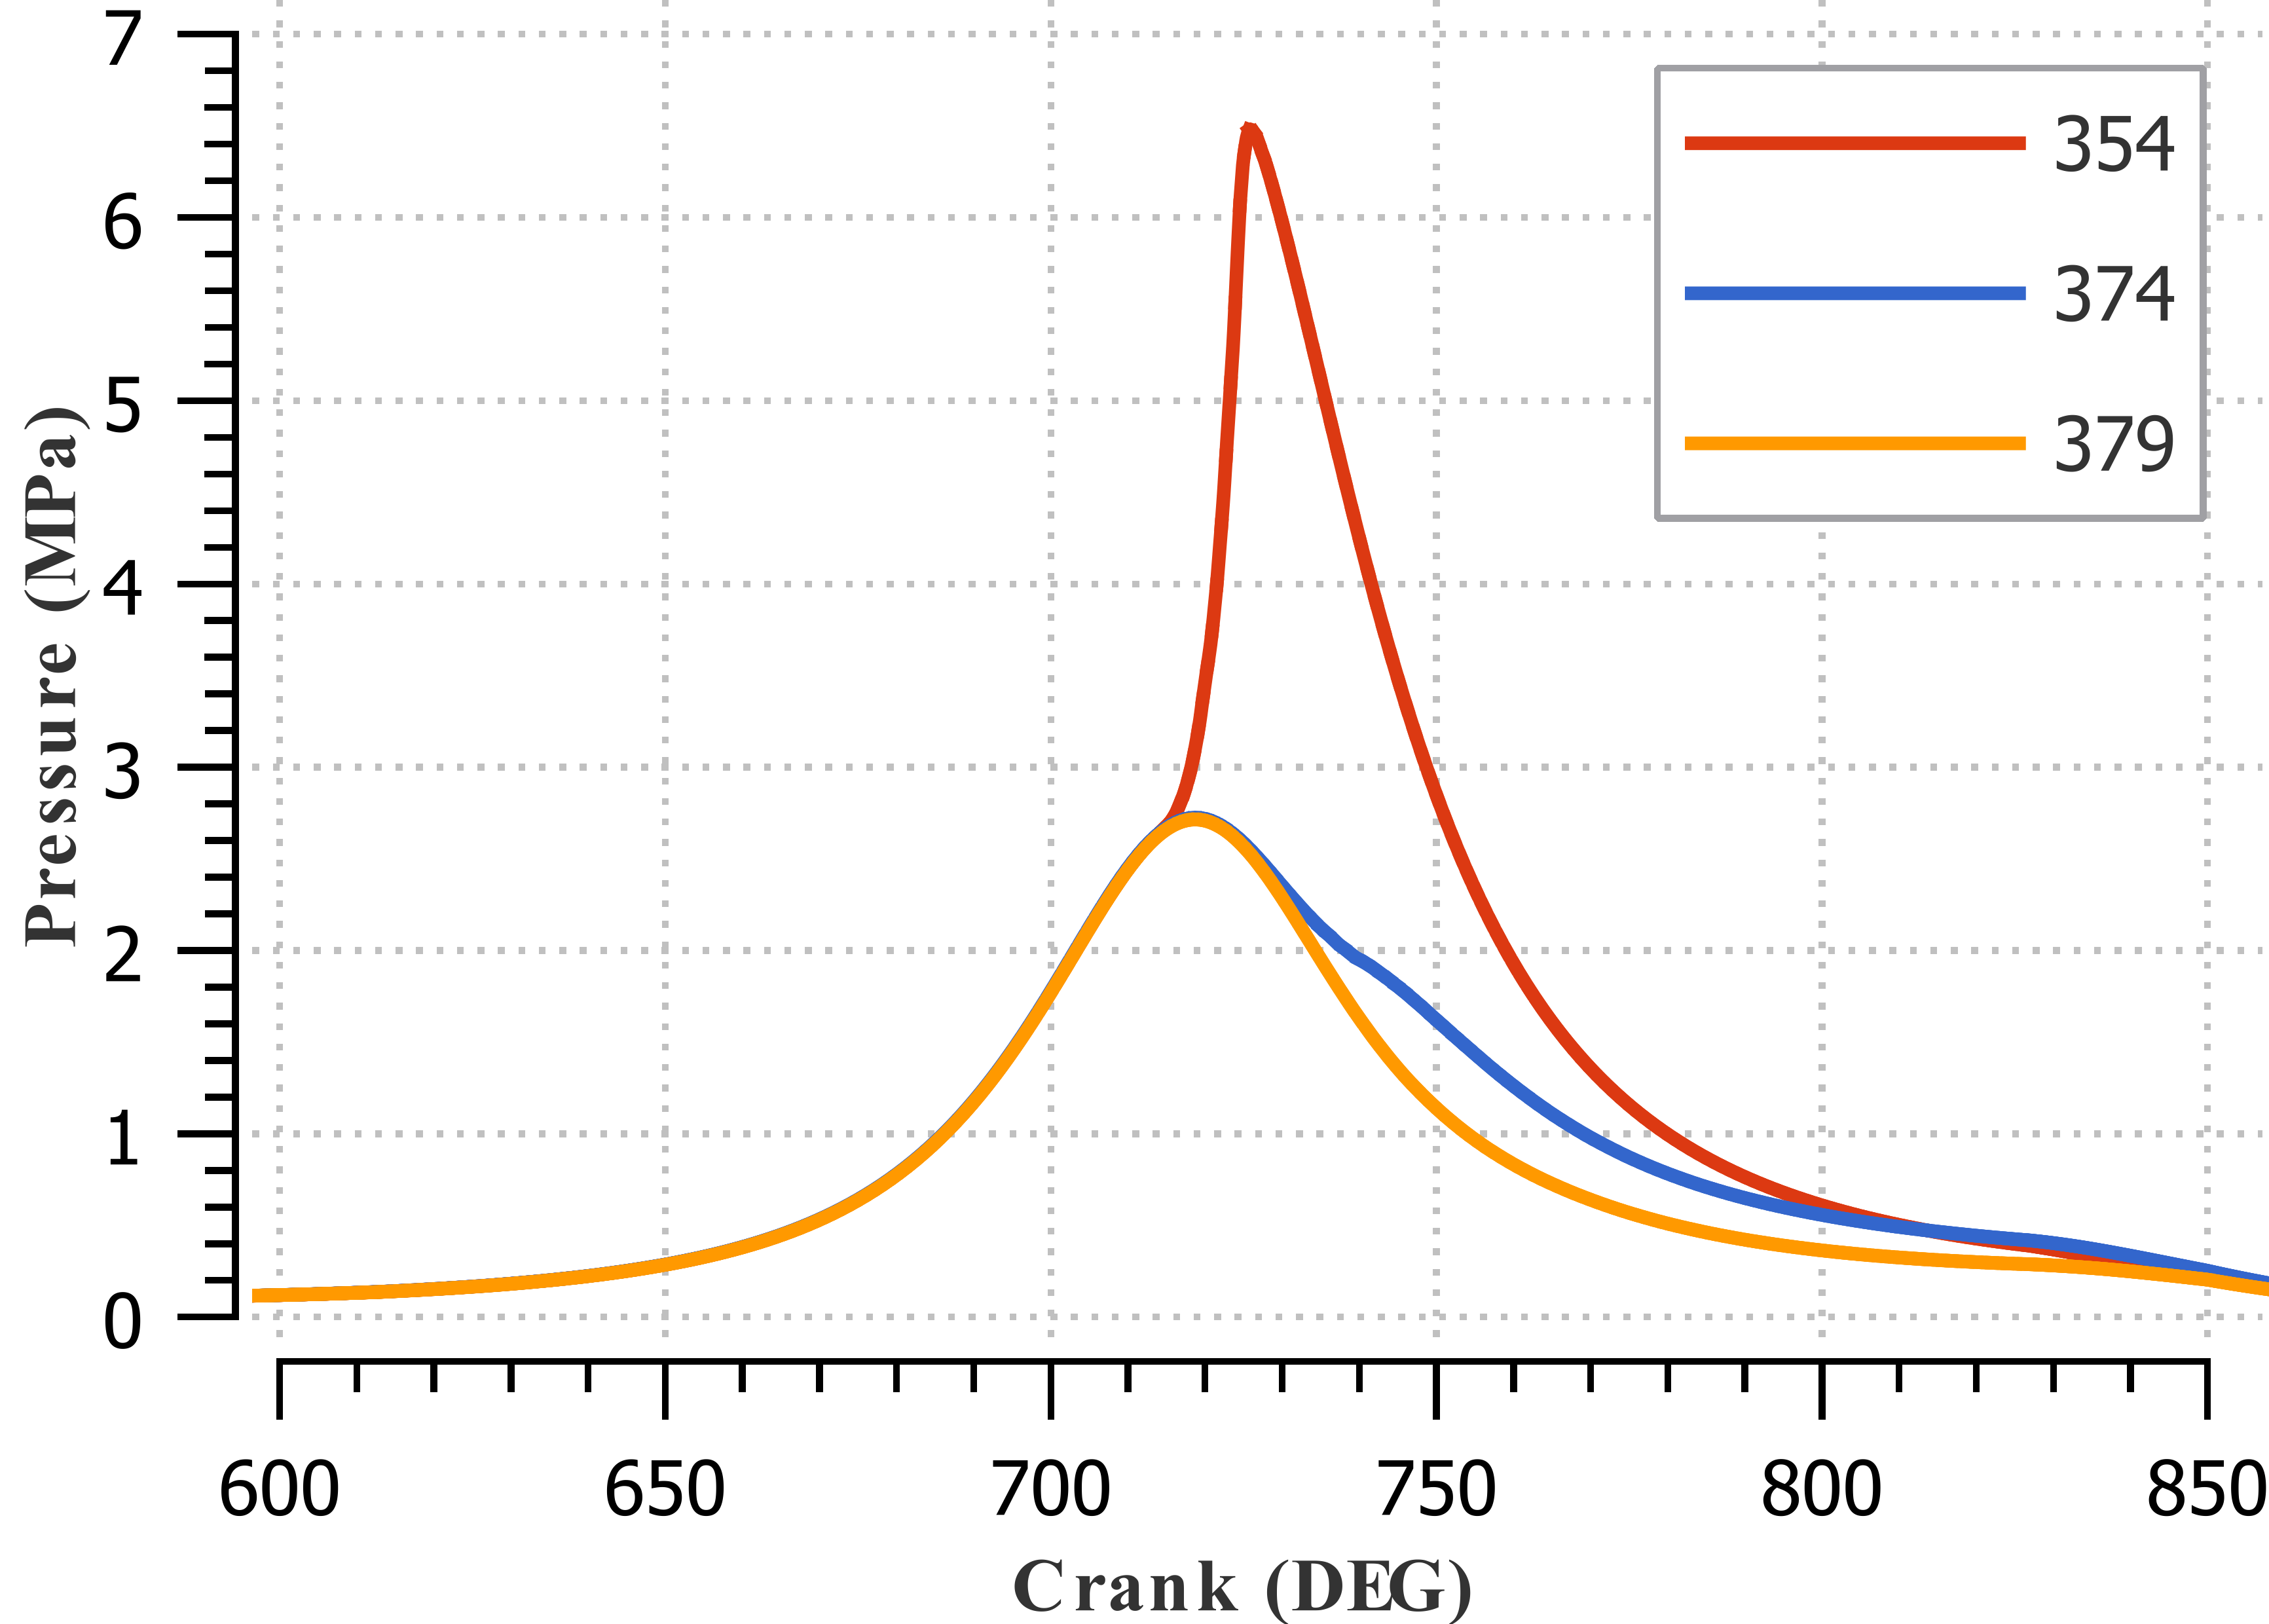
\includegraphics{Plots/30_pressure.png}}
    \caption{In-Cylinder Pressure for VOT = 30}
    \label{plt_tttt}
    \end{figure}

\begin{figure}[htbp]
    \centerline{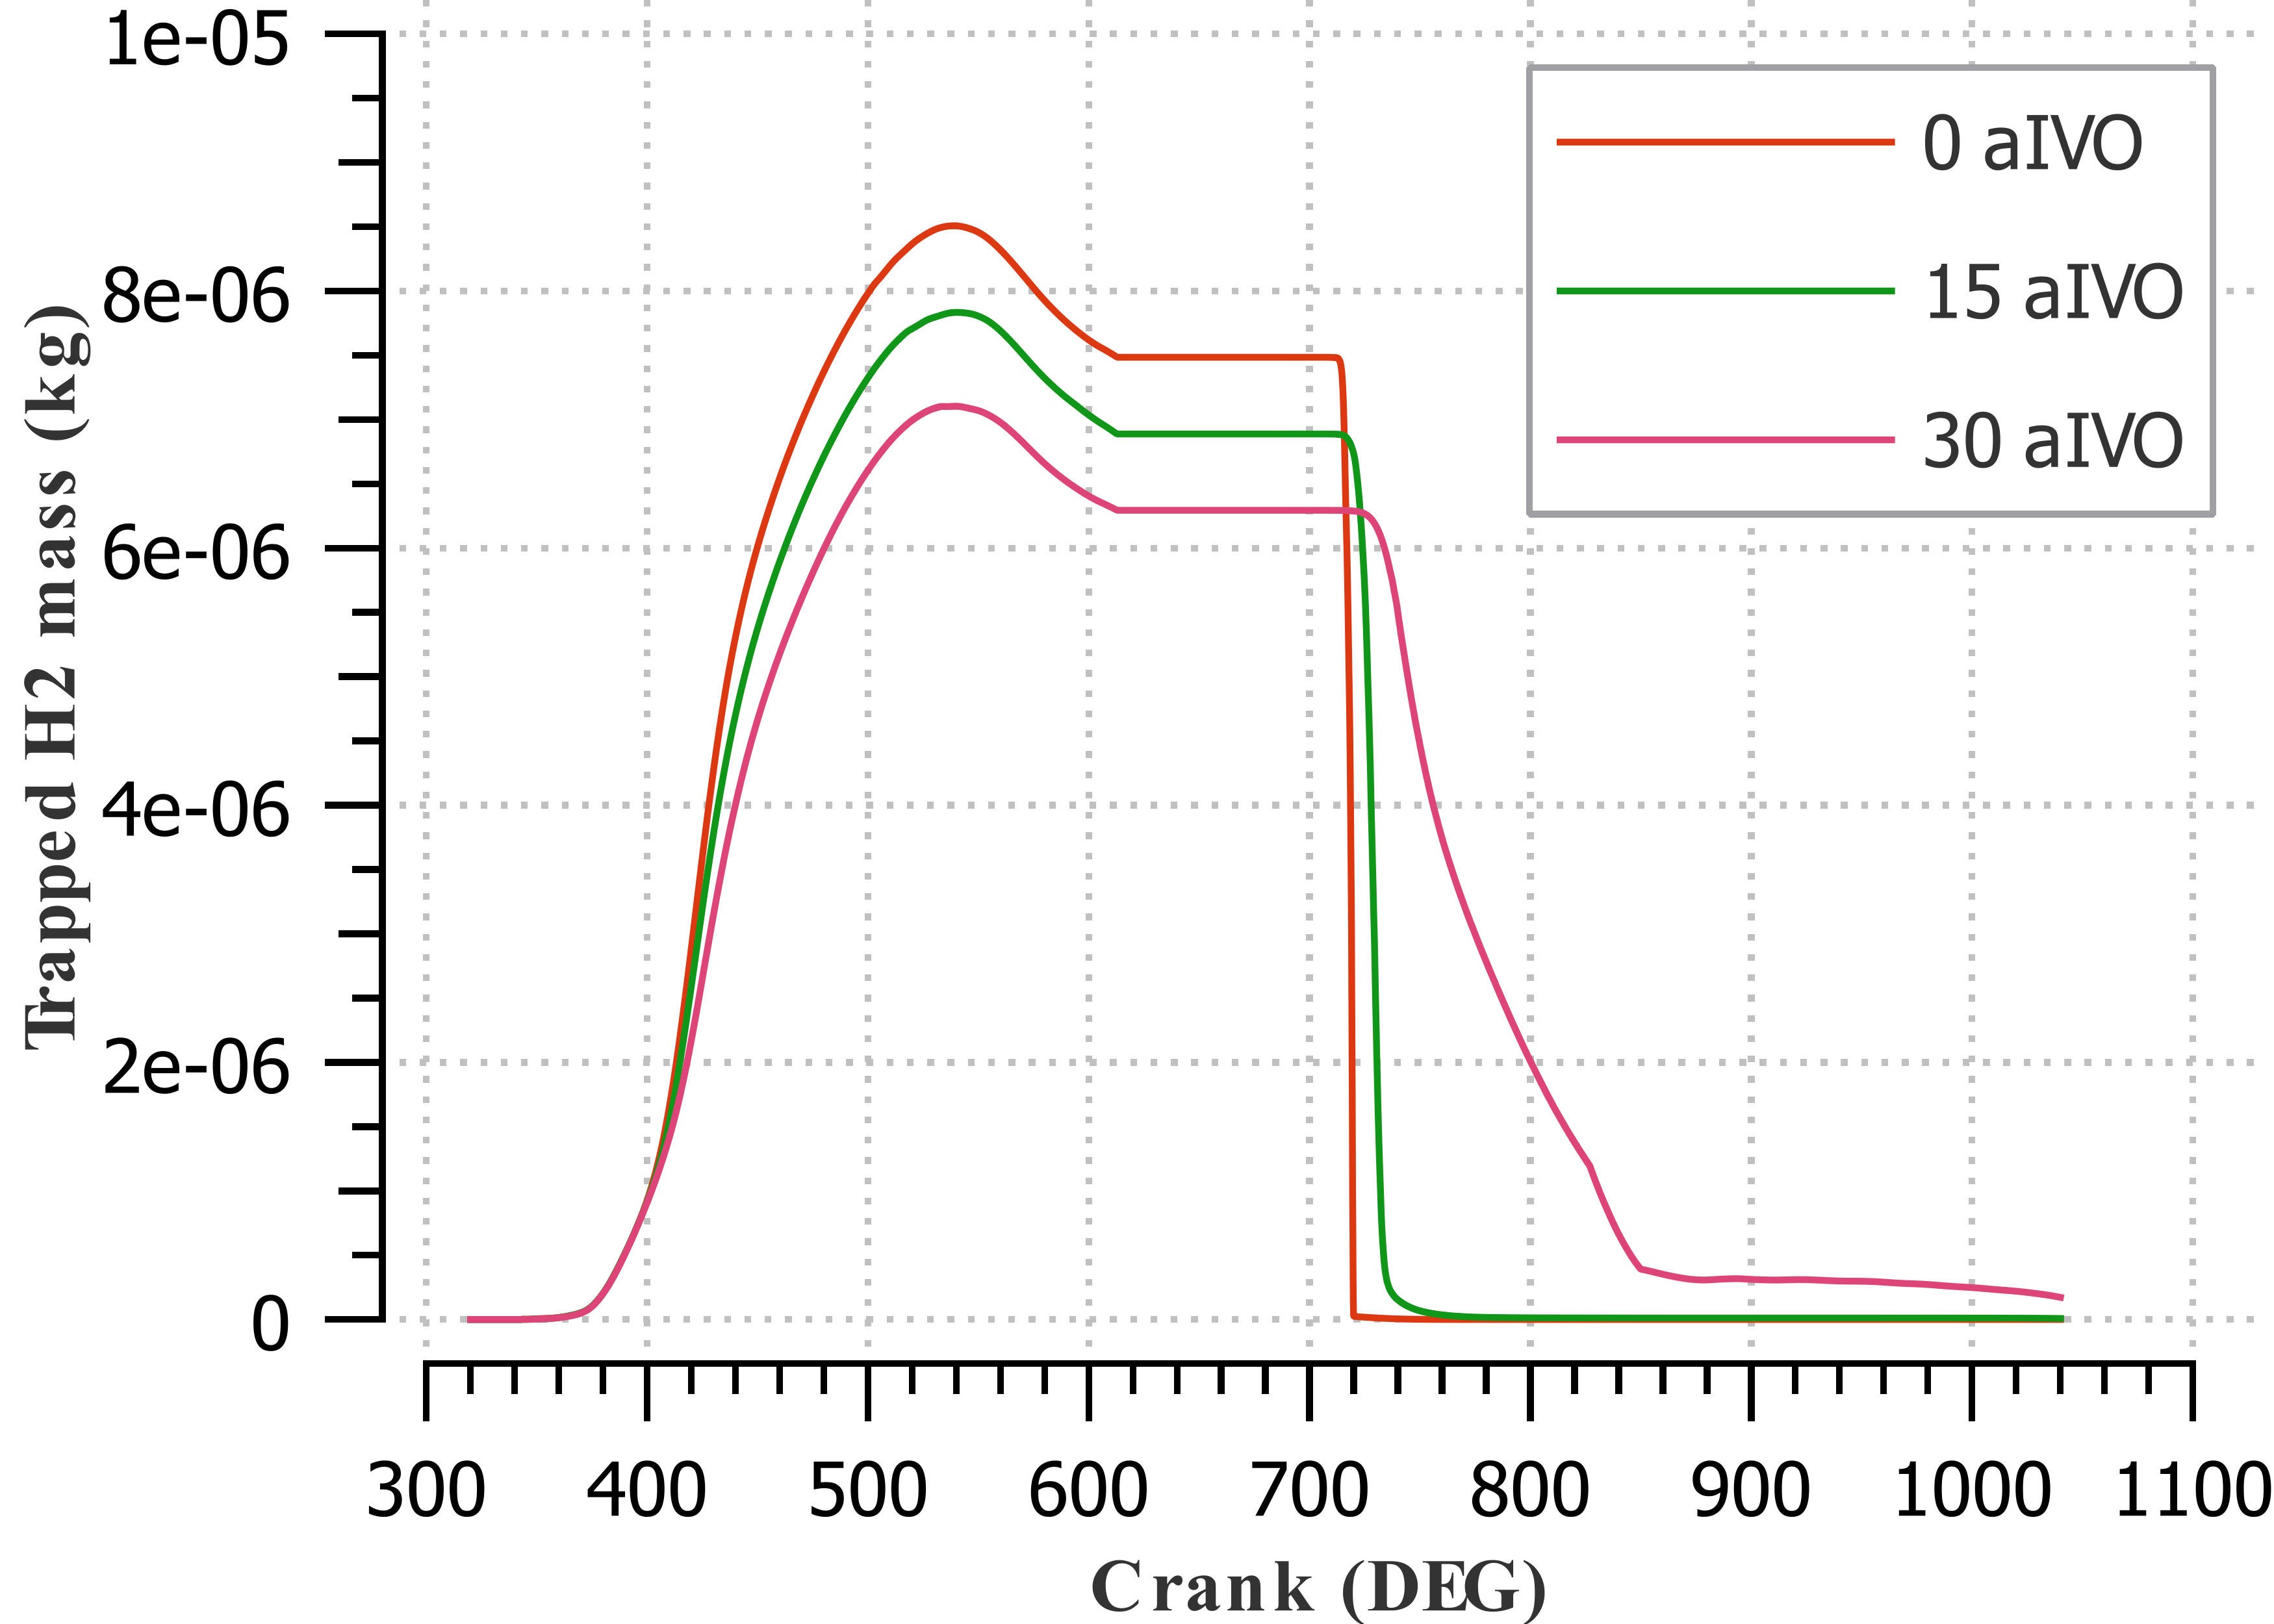
\includegraphics[width=88.9mm]{Plots/30_h2.png}}
    \caption{Trapped Mass for VOT = 30}
    \label{plt_ttt}
    \end{figure}



\subsection{Combustion Simulations}

\section{Results}
\subsection{Trapped Mass}
As we can see on the graph trapped hydrogen mass reduces with delaying injection delay. In the early injection, the injected hydrogen of per cycle can fully flow into the cylinder rapidly. But delayed injection time, the hydrogen gas injected per cycle could not fully enter the cylinder. 

\begin{figure}[htbp]
    \centerline{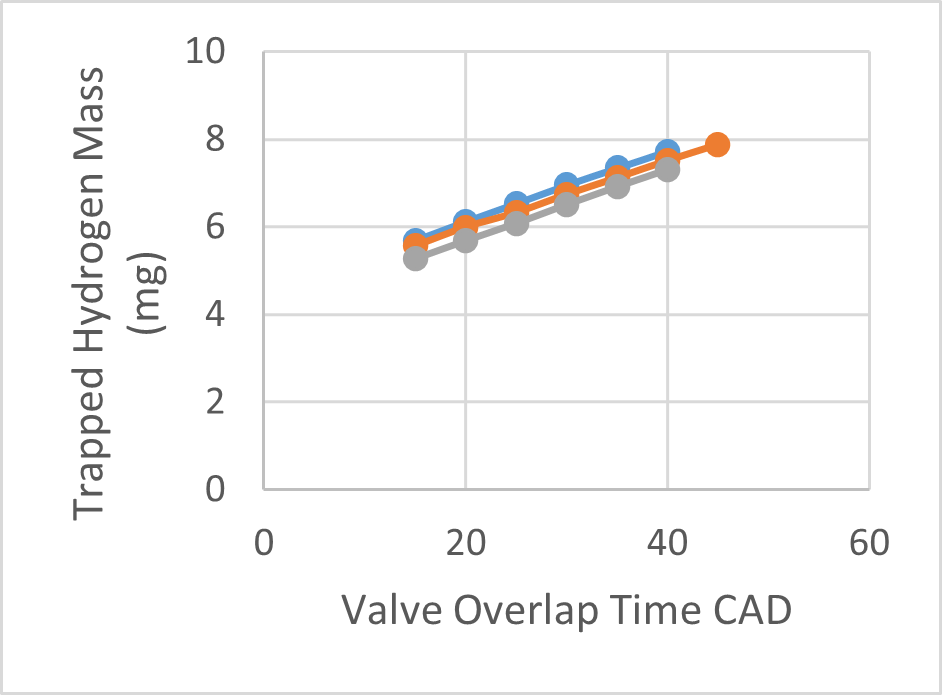
\includegraphics{Plots/trapped mass.png}}
    \caption{Trapped Hydrogen Mass}
    \label{plt_1}
    \end{figure}

\subsection{In-Cylinder Pressure}
\begin{figure}[htbp]
    \centerline{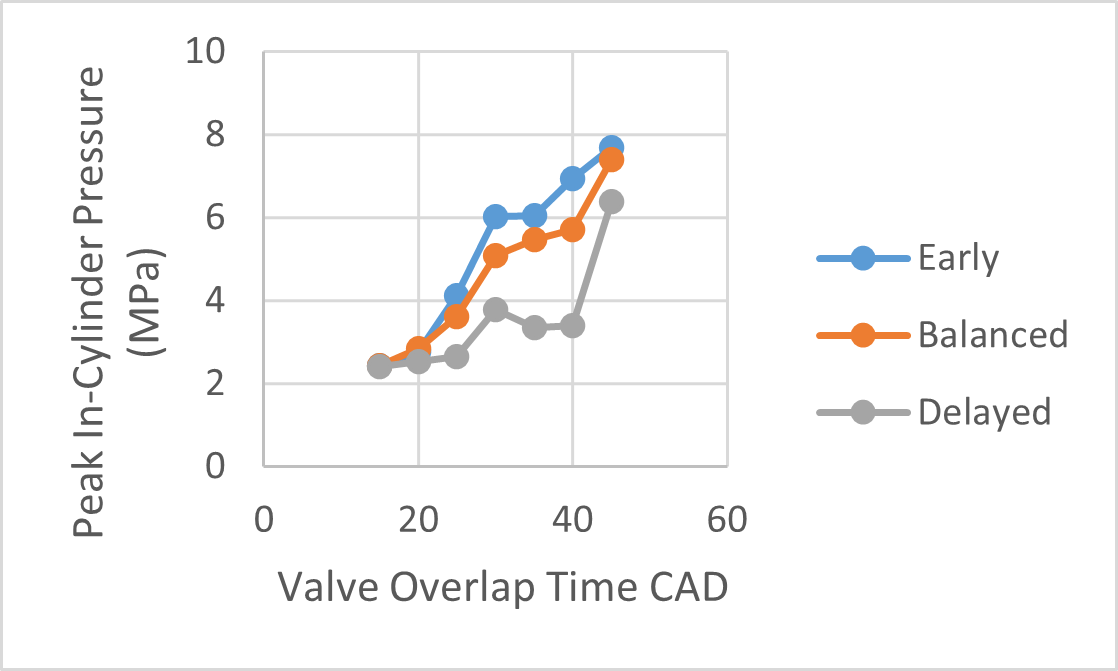
\includegraphics{Plots/pressure.png}}
    \caption{Pressure}
    \label{plt_2}
    \end{figure}

\subsection{In-Cylinder Temperature}
\begin{figure}[htbp]
    \centerline{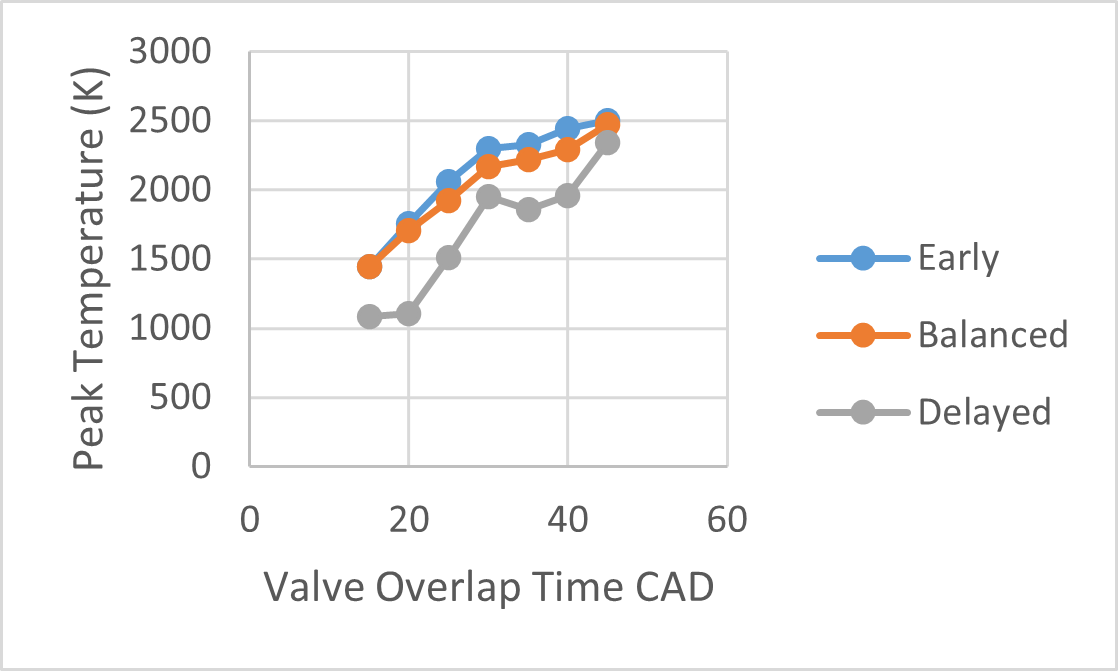
\includegraphics{Plots/temperature.png}}
    \caption{Temperature}
    \label{plt_3}
    \end{figure}

\subsection{Peak Heat Release Rate}
\begin{figure}[htbp]
    \centerline{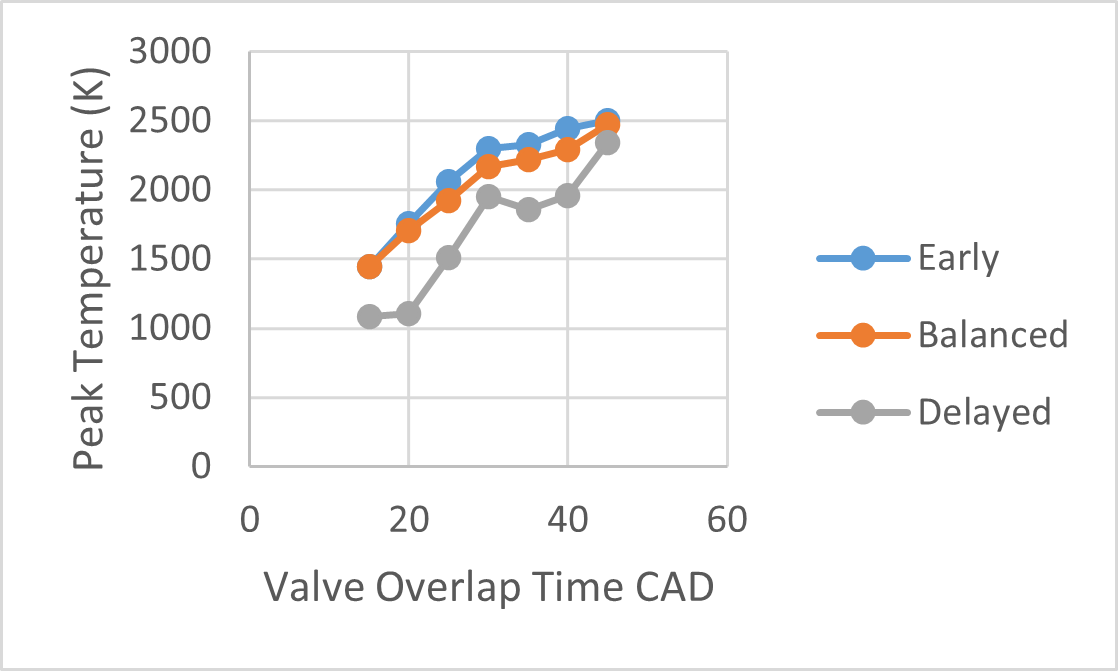
\includegraphics{Plots/hrr.png}}
    \caption{HRR}
    \label{plt_4}
    \end{figure}

Low heat release rate indicates slower rate of chemical reaction while high heat release rate indicates rapid combustion. To produce more useful work from the combustion process, gradual combustion process should be ensured. 
HRR < x can be defined as incomplete combustion and HRR > y can be defined as knocking combustion. Both of which should be eliminated for an effective combustion process.
according to the results, xxxx cases can be defined as inefficient combustion cases.
This rapid burning is due to increased trapped mass within the cylinder and consequently increased equivalence ratios.
Ranges of valve and injection timing for proper combustion characteristics.

\subsection{IMEP}

\subsection{Peak Heat Release Rate}
\begin{figure}[htbp]
    \centerline{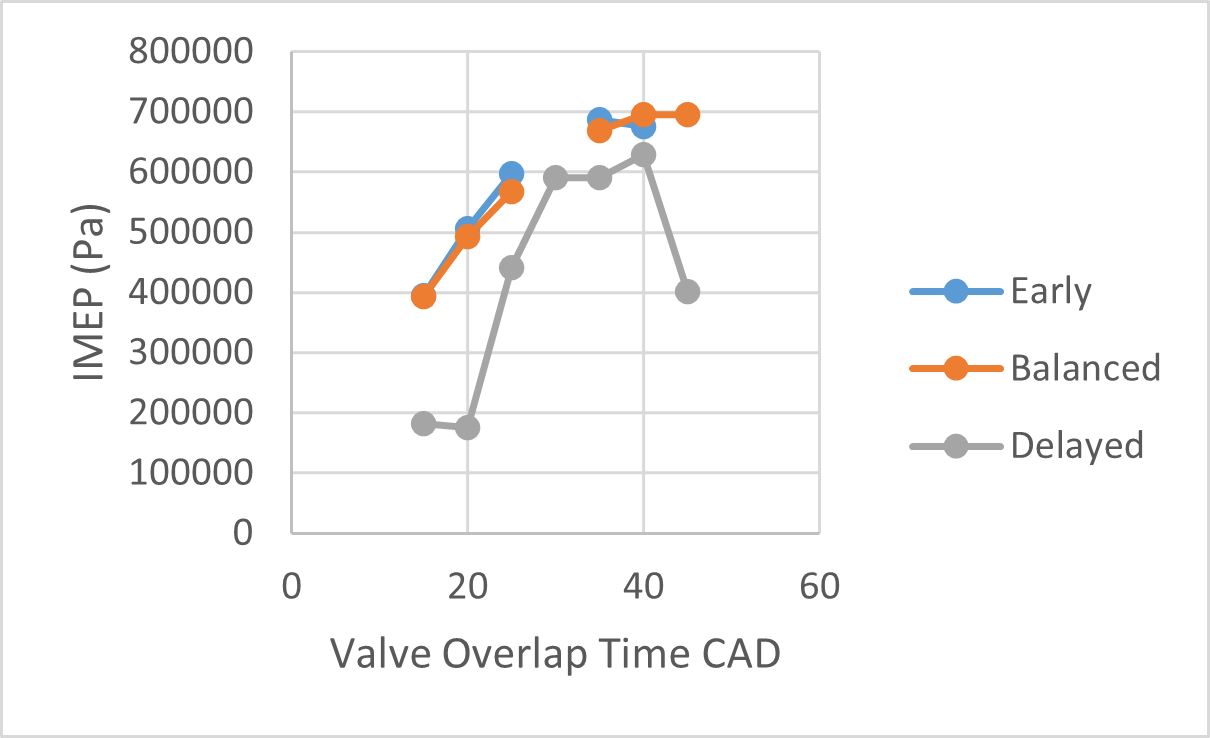
\includegraphics{Plots/imep.png}}
    \caption{IMEP}
    \label{plt_5}
    \end{figure}
Variation of IMEP with VOT and injection mode.
Reduced trapped mass – less time to go to cylinder.
    
\subsection{Efficiency}
\begin{figure}[htbp]
    \centerline{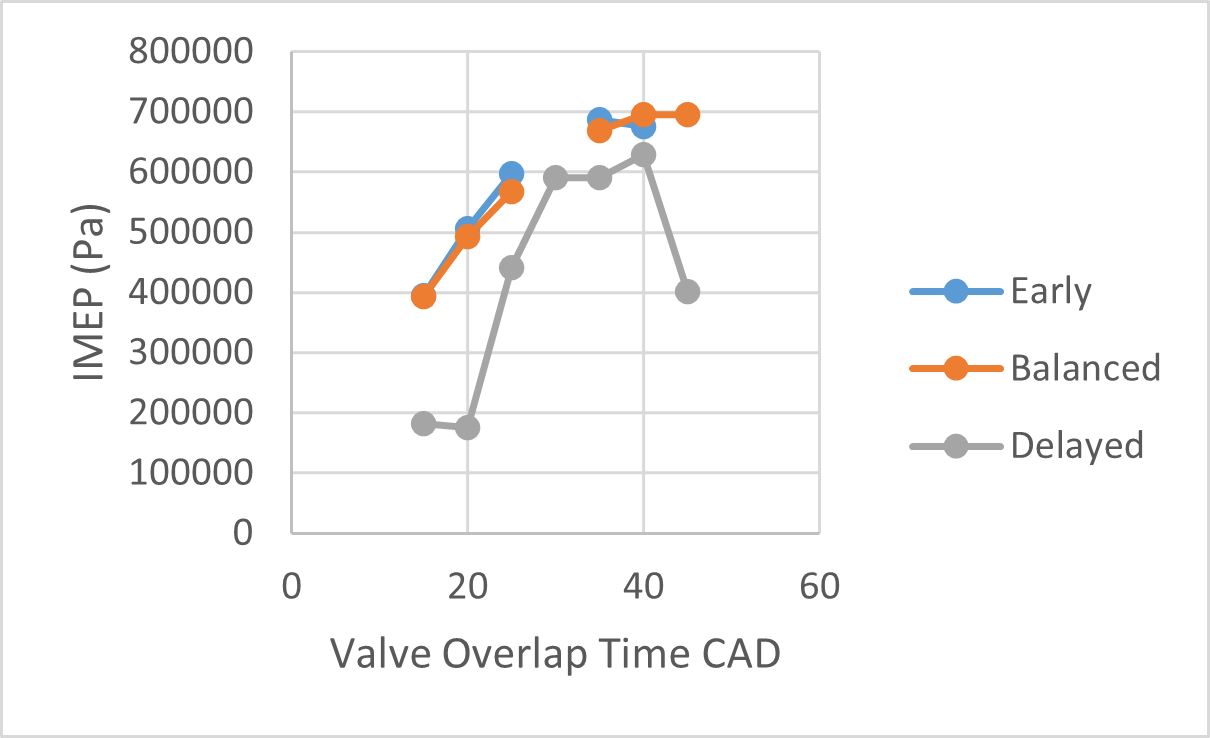
\includegraphics{Plots/imep.png}}
    \caption{Efficiency}
    \label{plt_6}
    \end{figure}
\subsection{Local Concentration}
\begin{figure}[htbp]
    \centerline{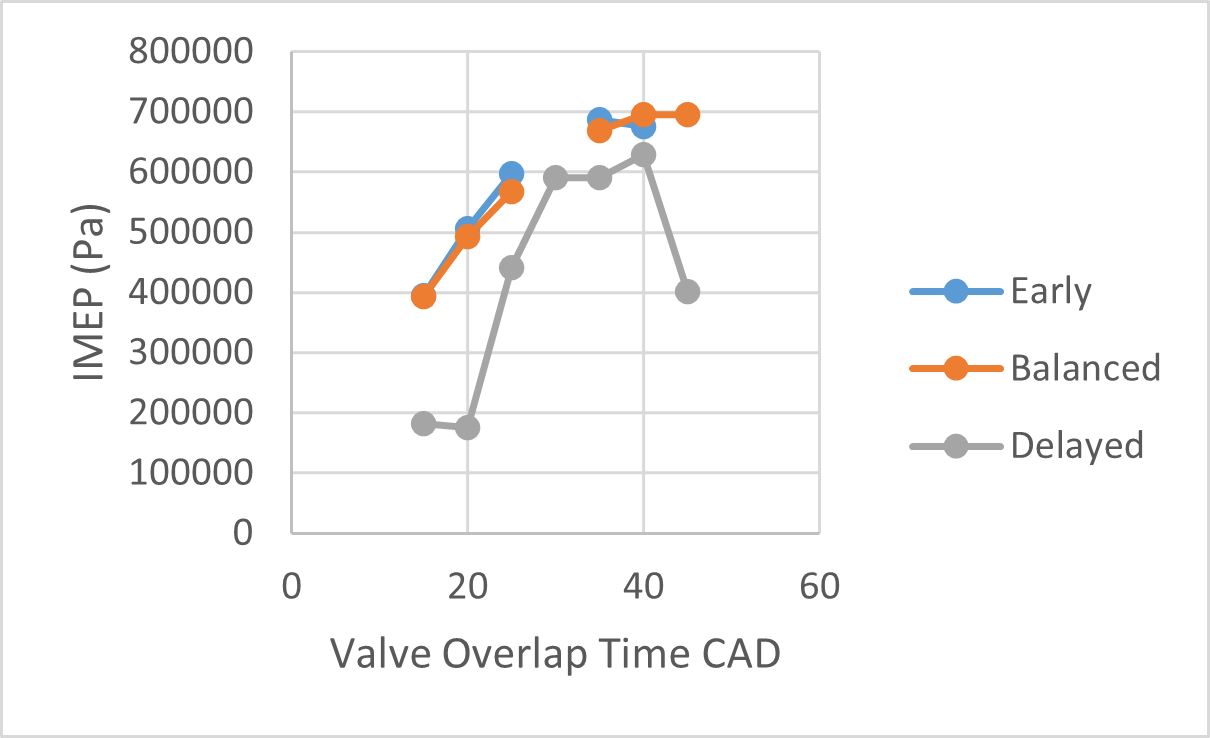
\includegraphics{Plots/imep.png}}
    \caption{Local Concentration}
    \label{plt_7}
    \end{figure}

\section{Conclusion}

\section{Future Works}
Effect of valve and injection timing on backfire, in particular, flame propagation.

\section*{Acknowledgment}



\begin{thebibliography}{00}
\bibitem{b1} G. Eason, B. Noble, and I. N. Sneddon, ``On certain integrals of Lipschitz-Hankel type involving products of Bessel functions,'' Phil. Trans. Roy. Soc. London, vol. A247, pp. 529--551, April 1955.
\bibitem{b2} J. Clerk Maxwell, A Treatise on Electricity and Magnetism, 3rd ed., vol. 2. Oxford: Clarendon, 1892, pp.68--73.
\bibitem{b3} I. S. Jacobs and C. P. Bean, ``Fine particles, thin films and exchange anisotropy,'' in Magnetism, vol. III, G. T. Rado and H. Suhl, Eds. New York: Academic, 1963, pp. 271--350.
\bibitem{b4} K. Elissa, ``Title of paper if known,'' unpublished.
\bibitem{b5} R. Nicole, ``Title of paper with only first word capitalized,'' J. Name Stand. Abbrev., in press.
\bibitem{b6} Y. Yorozu, M. Hirano, K. Oka, and Y. Tagawa, ``Electron spectroscopy studies on magneto-optical media and plastic substrate interface,'' IEEE Transl. J. Magn. Japan, vol. 2, pp. 740--741, August 1987 [Digests 9th Annual Conf. Magnetics Japan, p. 301, 1982].
\bibitem{b7} M. Young, The Technical Writer's Handbook. Mill Valley, CA: University Science, 1989.
\end{thebibliography}

\end{document}
